
\section{Magic Overview}
\label{sec:MagicOverview}
Magical powers spring from the rotations of the planes, the souls of living creatures, the will of the deities,
and more mysterious sources still.
It is a virtually omnipresent power, as real as muscle and steel.

Even an undead creature or a being that has no physical form can have the reserve of inner strength necessary to cast spells, 
as long as it has an Intelligence score of at least 1. %Vermin possessed of a hive mind ability are an exception to this rule.

A spell is a one-time magical effect. 

Spellcasting characters and creatures need not prepare their spells for use ahead of time. 
They either have sufficient spell points to cast a spell, or they do not.
A spell is cast when a spellcasting character pays its spell point cost. 
Some innately magical creatures automatically cast spells, called spell-like abilities, without paying a spell point cost. 
Other creatures pay spell points to cast their spells, just as characters do.

Each spell has a specific effect. A spell known to a spellcasting character can be used whenever he or she can spend the spell points to pay for it.

Magic has one fundamental rule. This most fundamental rule of magic is as follows:
\begin{quote}
\Large{The maximum number of spell points you can spend on a spell is equal to your caster level.}
\end{quote}
Spell points and caster levels are explained in detail below.
\subsection{Casting Spells}
Spellcasting characters and magical creatures cast spells. 
Whether they cost spell points when cast by a spellcasting character, or are cast as spell-like abilities, spells' effects remain the same.
\subsubsection{Choosing a Spell}
First you must choose which spell to cast. 
You can select any spell you know, provided you are capable of casting spells of that level or higher. 
To cast a spell, you must pay spell points, which count against your daily total. 
You can cast the same spell multiple times if you have points left to pay for it.

\subsubsection{Concentration}
To cast a spell, you must concentrate. If something threatens to interrupt your concentration while you're casting a spell, you must succeed on a \nameref{sec:Concentration} check or lose the spell points without casting the spell. 
The more distracting the interruption and the higher the level of the spell that you are trying to cast, the higher the DC. 
(Higher-level spells require more mental effort.)

\paragraph{Injury:} Getting hurt or being affected by hostile magic while trying to cast a spell can break your concentration and ruin a spell. 
If you take damage while trying to cast a spell, you must make a \nameref{sec:Concentration} check (DC 10 + points of damage taken + the level of the spell you're casting). 
The interrupting event strikes during casting if it occurs between when you start and when you complete casting a spell (for a spell with a casting time of 1 round or longer) or if it comes in response to your casting the spell (such as an attack of opportunity provoked by the casting of the spell or a contingent attack from a readied action).
If you are taking continuous damage half the damage is considered to take place while you are casting a spell. 
You must make a Concentration check (DC 10 + 1/2 the damage that the continuous source last dealt + the level of the spell you're casting).
If the last damage dealt was the last damage that the effect could deal then the damage is over, and it does not distract you.
Repeated damage does not count as continuous damage.

\paragraph{Spell:} If you are affected by a spell while attempting to cast a spell of your own, you must make a \nameref{sec:Concentration} check or lose the spell you are casting.
If the spell affecting you deals damage, the Concentration DC is 10 + points of damage + the level of the spell you're casting. 
If the spell interferes with you or distracts you in some other way, the Concentration DC is the spell's save DC + the level of the spell you're casting. 
For a spell with no saving throw, it's the DC that the spell's saving throw would have if a save were allowed.

\paragraph{Grappling or Pinned:} To cast a spell while grappling or pinned, you must make a \nameref{sec:Concentration} check (DC 20 + the level of the spell you're casting) or lose the spell. 
You cannot provide a somatic component (see components, below) while grappling, and if pinned, you may not be able to provide a verbal component, at the option of the creature that has you pinned.

\paragraph{Vigorous Motion:} If you are riding on a moving mount, taking a bouncy ride in a wagon, on a small boat in rough water, belowdecks in a storm-tossed ship, or simply being jostled in a similar fashion, you must make a \nameref{sec:Concentration} check (DC 10 + the level of the spell you're casting) or lose the spell.

\paragraph{Violent Motion:} If you are on a galloping horse, taking a very rough ride in a wagon, on a small boat in rapids or in a storm, on deck in a storm-tossed ship, or being tossed roughly about in a similar fashion, you must make a \nameref{sec:Concentration} check (DC 15 + the level of the spell you're casting) or lose the spell.

\paragraph{Violent Weather:} If you are in a high wind carrying blinding rain or sleet, the DC is 5 + the level of the spell you're casting. If you are in wind-driven hail, dust, or debris, the DC is 10 + the level of the spell you're casting. In either case, you lose the spell if you fail the \nameref{sec:Concentration} check. If the weather is caused by a spell, use the rules in the spell subsection above.

\paragraph{Casting spells on the Defensive:} If you want to cast a spell without provoking attacks of opportunity, you need to dodge and weave. You must make a \nameref{sec:Concentration} check (DC 15 + the level of the spell you're casting) to succeed. You lose the spell points without successful casting it if you fail.

\paragraph{Entangled:} If you want to cast a spell while entangled in a net or while affected by a spell with similar effects you must make a DC 15 \nameref{sec:Concentration} check to cast the spell. You lose the spell if you fail.

\subsubsection{Counterspells}
\label{sec:Counterspells}
It is possible to cast any spell as a counterspell. 
By doing so, you are using the spell's energy to disrupt the casting of the same spell by another character. 
Counterspelling works even if one spell is divine and the other arcane.

\paragraph{How Counterspells Work}
To use a counterspell, you must select an opponent as the target of the counterspell. 
You do this by choosing the ready action. 
In doing so, you elect to wait to complete your action until your opponent tries to cast a spell. 
(You may still move your speed, since ready is a standard action.)

If the target of your counterspell tries to cast a spell, make a \nameref{sec:Spellcraft} check (DC 15 + the spell's level). 
This check is a free action. 
If the check succeeds, you correctly identify the opponent's spell and can attempt to counter it. 
If the check fails, you can't do either of these things.

To complete the action, you must then cast the correct spell.
As a general rule, a spell can only counter itself. 
If you are able to cast the same spell you cast it, altering it slightly to create a counterspell effect. 
If the target is within range of the spell, both spells automatically negate each other with no other results.

\paragraph{Counterspelling Metamagic Spells and Augmented Spells}
Augments and metamagic feats are not taken into account when determining whether a spell can be countered.
You do not need to match the opponent's spell augments or metamagic applications.

\paragraph{Dispel Magic as a Counterspell}
You can use \nameref{Spell:DispelMagic} to counterspell another spellcaster, and you don't need to identify the spell he or she is casting. 
However, \nameref{Spell:DispelMagic} doesn't always work as a counterspell.

\subsubsection{Caster Level}
The variables of a spell's effect often depend on its caster level, which is (usually) equal to your spellcasting class level. 
A spell that can be augmented for additional effect is also limited by your caster level (you can't spend more spell points on a spell than your caster level). 
See \nameref{sec:Augment}, below.
You can cast a spell at a lower caster level than normal, but the caster level must be high enough for you to cast the spell in question, and all level-dependent features must be based on the same caster level.
In the event that a class feature or other special ability provides an adjustment to your caster level, this adjustment applies not only to all effects based on caster level (such as range, duration, and augmentation potential) but also to your caster level check to overcome your target's spell resistance and to the caster level used in dispel checks (both the dispel check and the DC of the check).

\subsubsection{Spell Failure}
If you try to cast a spell in conditions where the characteristics of the spell (range, area, and so on) cannot be made to conform, the spell fails and the spell points are wasted. 
Spells also fail if your concentration is broken (see \nameref{sec:Concentration}, above).

\subsubsection{The Spell's Result}
Once you know which creatures (or objects or areas) are affected, and whether those creatures have made successful saving throws (if any were allowed), you can apply whatever results a spell entails.

\subsubsection{Special Spell Effects}
Certain special features apply to all spells.

\paragraph{Attacks:} Some spells refer to attacking. 
All offensive combat actions, even those that don't damage opponents, such as disarm and bull rush, are considered attacks. 
All spells that opponents can resist with saving throws, that deal damage, or that otherwise harm or hamper subjects are considered attacks. 
\nameref{Spell:SummonMonster} and similar spells are not considered attacks because the spells themselves don't harm anyone.

\paragraph{Bonus Types:} Many spells give creatures bonuses to ability scores, Armor Class, attacks, and other attributes. 
Each bonus has a type that indicates how the spell grants the bonus. 
The important aspect of bonus types is that two bonuses of the same type don't generally stack. 
With the exception of dodge bonuses, most circumstance bonuses, and racial bonuses, only the better bonus works (see \nameref{sec:CombiningMagicalEffects}).
The same principle applies to penalties - a character taking two or more penalties of the same type applies only the worst one.
If the type of a bonus is not specified, it is an ``untyped'' bonus, which stacks with everything but another instance of what granted the untyped bonus.

\paragraph{Bringing Back the Dead:} Some powerful spells have the ability to restore slain characters to life. 
When a living creature dies, its soul departs the body, leaves the Material Plane, travels through the Astral Plane, and goes to abide on the plane where the creature's deity resides. 
If the creature did not worship a deity, its soul departs to the plane corresponding to its alignment. 
Bringing someone back from the dead means retrieving his or her soul and returning it to his or her body.

\subparagraph{Level Loss:} The passage from life to death and back again is a wrenching journey for a being's soul. 
Consequently, any creature brought back to life usually loses one level of experience.
The character's new experience point total is midway between the minimum needed for his or her new (reduced) level and the minimum needed for the next one. 
If the character was 1st level at the time of death, he or she loses 2 points of Constitution instead of losing a level. 
This level loss or Constitution loss cannot be repaired by any mortal means, even the spells \nameref{Spell:Wish} or \nameref{Spell:Miracle}. 
A revived character can regain a lost level by earning XP through further adventuring. 
A revived character who was 1st level at the time of death can regain lost points of Constitution by improving his or her Constitution score when he or she attains a level that allows an ability score increase.

\subparagraph{Memory Loss:} A character brought back from the dead has barely any memories relating to its afterlife. At most, a vague sensation of what the deity's plane felt like remains.

\subparagraph{Preventing Revivification:} 
Enemies can take steps to make it more difficult for a character to be returned from the dead. 
Keeping the body being the most elementary, though the most powerful of spellcasters can bypass this limitation. 
See individual spell descriptions.

\subparagraph{Revivification Against One's Will:} 
A soul knows the name, alignment, and patron deity (if any) of the character attempting to revive it and may refuse to return on that basis.
Only the foulest magic can return a soul to life if it does not wish to be.
\subsubsection{Combining Magical Effects}
\label{sec:CombiningMagicalEffects}
\paragraph{Psionics-Magic Transparency:} The default rule for the interaction of psionics and magic is simple: 
Powers interact with spells and spells interact with powers in the same way a spell or normal spell-like ability interacts with another spell or spell-like ability. 
This is known as psionics-magic transparency.
Though not explicitly called out in the spell descriptions or magic item descriptions, spells, spell-like abilities, and magic items that could potentially affect psionics do affect psionics. 
When the rule about psionics-magic transparency is in effect, it has the following ramifications:
\begin{itemize}
\item Spell resistance is effective against powers, using the same mechanics. 
Likewise, power resistance is effective against spells, using the same mechanics as spell resistance. 
If a creature has one kind of resistance, it is assumed to have the other. (The effects have similar ends despite having been brought about by different means.)
\item All spells that dispel magic (such as \nameref{Spell:DispelMagic}) have equal effect against powers of the same level using the same mechanics, and vice versa.
\item The spell \nameref{Spell:DetectMagic} detects powers as if they were spells.
\item Dead magic areas are also dead psionics areas.
\end{itemize}
\paragraph{Multiple Effects:} Spells or magical effects usually work as described no matter how many other spells or magical effects happen to be operating in the same area or on the same recipient. 
Except in special cases, a spell does not affect the way another spell operates. 
Whenever a spell has a specific effect on other spells, the spell description explains the effect (and vice versa for spells that affect spells). 
Several other general rules apply when spells or magical effects operate in the same place.

\paragraph{Stacking Effects:} Spells that provide bonuses or penalties on attack rolls, damage rolls, saving throws, and other attributes usually do not stack with themselves. 
More generally, two bonuses of the same type don't stack even if they come from different spells. 
You use whichever bonus gives you the better result. 

\paragraph{Different Bonus Types:} The bonuses or penalties from two different spells stack if the effects are of different types. 
A bonus that isn't named (just a ``+2 bonus`` rather than a ``+2 insight bonus'') stacks with any bonus but another instance of the same effect that granted the bonus.

\paragraph{Same Effect More than Once in Different Strengths:} 
In cases when two or more similar or identical effects are operating in the same area or on the same target, but at different strengths, only the best one applies. 
If one spell is dispelled or its duration runs out, the other spell remains in effect (assuming its duration has not yet expired).

\paragraph{Same Effect with Differing Results:} 
The same spell can sometimes produce varying effects if applied to the same recipient more than once. 
The last effect in a series trumps the others. 
None of the previous spells are actually removed or dispelled, but their effects become irrelevant while the final spell in the series lasts.

\paragraph{One Effect Makes Another Irrelevant:} Sometimes, a spell can render another spell irrelevant.

\subparagraph{Multiple Mental Control Effects:} Sometimes magical effects that establish mental control render one another irrelevant. 
Mental controls that don't remove the recipient's ability to act usually do not interfere with one another, though one may modify another. If a creature is under the control of two or more creatures, it tends to obey each to the best of its ability, and to the extent of the control each effect allows. 
If the controlled creature receives conflicting orders simultaneously, the competing controllers must make opposed Charisma checks to determine which one the creature obeys.

\subparagraph{Spells with Opposite Effects:} Spells with opposite effects apply normally, with all bonuses, penalties, or changes accruing in the order that they apply.
Some spells negate or counter each other. This is a special effect that is noted in a spell's description.

\paragraph{Instantaneous Effects:} Two or more magical effects with instantaneous durations work cumulatively when they affect the same object, place, or creature.

\subsection{The Spell Point Reserve}
Spellcasting characters fuel their abilities through a pool, or reserve, of spell points. 
Your spell point reserve is equal to your base spell points gained from your class\footnote{
Individual class tables contain information on how many spell points are granted by that class. However, the mathematically inclined may be interested in the formulas behind the tables:
\begin{itemize}
 \item The Bard has $\lfloor\frac{\text{level}^2}{2}\rfloor$ base SP/day.
 \item The Cleric and Wizard have $\lceil (\text{level}^2+\text{level}+1) \cdot \frac{3}{4}\rceil$ base SP/day.
 \item The Sorcerer has $\lceil \text{level}^2+\text{level}+1 \rceil$ base SP/day.
 \item The Paladin and Ranger progressions are not known to me, as they emulate the Psychic Warrior progression. Polynomial fitting has not been fruitful.
\end{itemize}
In all the formulas, ``level'' refers to the class level of the spellcasting class in question.}, bonus spell points from a high key ability score (see Abilities and Spellcasters, below), and any additional bonus spell points from sources such as your character race and feat selections.
\subsubsection{Multiclass Spellcasting Characters}
If you have levels in more than one spellcasting class, you combine your spell points from each class to make up your reserve. 
You can use these spell points to cast spells from any spellcasting class you have. 
While you maintain a single reserve of spell points from your class, race, and feat selections, you are still limited by the caster level you have achieved with each spell you know. 
\subsubsection{Abilities and spellcasters}
The ability that your spells depend on - your key ability score as a spellcaster - is related to what spellcasting class (or classes) you have levels in, as detailed for each individual spellcasting class.
The modifier for this ability is referred to as your key ability modifier. 
If your character's key ability score is 9 or lower, you can't cast spells from that spellcasting class.

\textbf{How To Determine Bonus Spell Points:} 
Your key ability score grants you additional spell points equal to 
\begin{quote}
\centering
\large 
 {your key ability modifier $\times$ your caster level $\times \frac{1}{2}$.}
\end{quote}
The results of this equation are summarized on the \nameref{tab:BonusSpellPoints} table.
\begin{table*}
\caption{Ability Modifiers and Bonus Spell Points}
\label{tab:BonusSpellPoints}
\makebox[\textwidth]{\resizebox{\textwidth}{!}{
\begin{tabular}{p{0.06\textwidth}*{19}{p{0.025\textwidth}}p{0.03\textwidth}}
\toprule
Ability&\multicolumn{20}{c}{Bonus Spell Points (by Caster Level)}\\
Score&	1st&	2nd&	3rd&	4th&	5th&	6th&	7th&	8th&	9th&	10th&	11th&	12th&	13th&	14th&	15th&	16th&	17th&	18th&	19th&	20th\\
\midrule
10-11&	0&	0&	0&	0&	0&	0&	0&	0&	0&	0&	0&	0&	0&	0&	0&	0&	0&	0&	0&	0\\
12-13&	0&	1&	1&	2&	2&	3&	3&	4&	4&	5&	5&	6&	6&	7&	7&	8&	8&	9&	9&	10\\
14-15&	1&	2&	3&	4&	5&	6&	7&	8&	9&	10&	11&	12&	13&	14&	15&	16&	17&	18&	19&	20\\
16-17&	1&	3&	4&	6&	7&	9&	10&	12&	13&	15&	16&	18&	19&	21&	22&	24&	25&	27&	28&	30\\
18-19&	2&	4&	6&	8&	10&	12&	14&	16&	18&	20&	22&	24&	26&	28&	30&	32&	34&	36&	38&	40\\
20-21&	2&	5&	7&	10&	12&	15&	17&	20&	22&	25&	27&	30&	32&	35&	37&	40&	42&	45&	47&	50\\
22-23&	3&	6&	9&	12&	15&	18&	21&	24&	27&	30&	33&	36&	39&	42&	45&	48&	51&	54&	57&	60\\
24-25&	3&	7&	10&	14&	17&	21&	24&	28&	31&	35&	38&	42&	45&	49&	52&	56&	59&	63&	66&	70\\
26-27&	4&	8&	12&	16&	20&	24&	28&	32&	36&	40&	44&	48&	52&	56&	60&	64&	68&	72&	76&	80\\
28-29&	4&	9&	13&	18&	22&	27&	31&	36&	40&	45&	49&	54&	58&	63&	67&	72&	76&	81&	85&	90\\
30-31&	5&	10&	15&	20&	25&	30&	35&	40&	45&	50&	55&	60&	65&	70&	75&	80&	85&	90&	95&	100\\
32-33&	5&	11&	16&	22&	27&	33&	38&	44&	49&	55&	60&	66&	71&	77&	82&	88&	93&	99&	104&	110\\
34-35&	6&	12&	18&	24&	30&	36&	42&	48&	54&	60&	66&	72&	78&	84&	90&	96&	102&	108&	114&	120\\
36-37&	6&	13&	19&	26&	32&	39&	45&	52&	58&	65&	71&	78&	84&	91&	97&	104&	110&	117&	123&	130\\
38-39&	7&	14&	21&	28&	35&	42&	49&	56&	63&	70&	77&	84&	91&	98&	105&	112&	119&	126&	133&	140\\
40-41&	7&	15&	22&	30&	37&	45&	52&	60&	67&	75&	82&	90&	97&	105&	112&	120&	127&	135&	142&	150\\
\bottomrule
\end{tabular}}}
\end{table*}
\subsubsection{Daily Spell Point Acquisition:}
\label{sec:DailySpellPointAcquisition}
To regain used daily spell points, a spellcasting character must have a clear mind. 
To clear his mind, he \footnote{A number of lines in this documents tend to assume that the character is male and if not human, at least humanoid-shaped.
This is because the document's original author is a human male who really didn't give gender-neutral language enough thought from the beginning.} must first sleep for 8 hours.
The character does not have to slumber for every minute of the time, but he must refrain from movement, combat, casting spells, skill use, conversation, or any other demanding physical or mental task during the rest period. 
If his rest is interrupted, each interruption adds 1 hour to the total amount of time he has to rest to clear his mind, and he must have at least 1 hour of rest immediately prior to regaining lost spell points. 
If the character does not need to sleep for some reason, he still must have 8 hours of restful calm before regaining spell points.

\paragraph{Recent Casting Limit/Rest Interruptions:} If a spellcasting character has cast spells recently, the drain on his resources reduces his capacity to regain spell points. 
When he regains spell points for the coming day, all spell points he has used within the last 8 hours count against his daily limit.

\paragraph{Peaceful Environment:} To regain spell points, a spellcasting character must have enough peace, quiet, and comfort to allow for proper concentration. 
The spellcasting character's surroundings need not be luxurious, but they must be free from overt distractions, such as combat raging nearby or other loud noises. 
Exposure to inclement weather prevents the necessary concentration, as does any injury or failed saving throw the character might incur while concentrating on regaining spell points.

\paragraph{Regaining Spell Points:} Once the character has rested in a suitable environment, it takes an act of concentration spanning 1 full round to regain all power points of the spellcasting character's daily limit. 
This can be an instant's meditation, a prayer to the character's deity, or any other minor ritual the character performs at the start of each day.

\paragraph{Death and Spell Points:} If a character dies, all daily spell points stored in his mind are wiped away. 
A potent effect (such as \nameref{Spell:Wish}) can recover the lost spell points when it recovers the character.
\subsubsection[Magical Focus]{Gain Magical Focus}

\begin{figure*}
  \caption{Wizard, Cleric and Sorcerer attempt to regain their Magical Focus.}
  \centering
    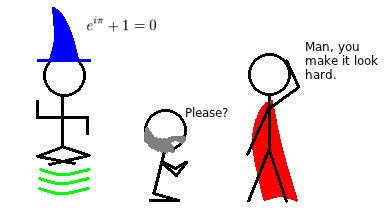
\includegraphics{Pics/SpellPoints.png}
\end{figure*}

\label{sec:MagicFocus}
Merely holding a reservoir of magical spell points in mind gives spellcasting characters a special energy. 
Spellcasting characters can put that energy to work without actually paying a spell point cost - they can become magically focused as a special use of the \nameref{sec:Concentration} skill.

If you have 1 or more spell points available, you can meditate to attempt to become magically focused. 
The DC to become magically focused is 20. Meditating is a full-round action that provokes attacks of opportunity. 
When you are magically focused, you can expend your focus on any single Concentration check you make thereafter. 
When you expend your focus in this manner, your Concentration check is treated as if you rolled a 15. 
It's like taking 10, except that the number you add to your Concentration modifier is 15. 
You can also expend your focus to gain the benefit of a magical feat - many magical feats are activated in this way.

Once you are magically focused, you remain focused until you expend your focus, become unconscious, or go to sleep (or enter a meditative trance, in the case of elves), or until your spell point reserve drops to 0.
\subsubsection{Using Stored Spell Points}
\label{sec:UsingStoredSpellPoints}
A variety of magical items exist to store spell points for later use, in particular a storage device called a \nameref{Item:PearlOfPower}. 
Regardless of what sort of item stores the spell points, all spellcasting characters must follow strict rules when tapping stored spell points.

\paragraph{A Single Source:} When using spell points from a storage item to cast a spell, a spellcasting character may not pay the spell's cost with spell points from more than one source. 
He must either use an item, his own spell point reserve, or some other discrete spell point source to pay the casting cost. 

\paragraph{Recharging:} Most spell point storage devices allow spellcasting characters to ``recharge`` the item with their own spell points. 
Doing this depletes the character's spell point reserve on a 1-for-1 basis as if he had casted a spell; however, those spell points remain indefinitely stored. 
The opposite is not true - spellcasting characters may not use spell points stored in a storage item to replenish their own spell point reserves.
\subsection{Adding Spells}
Spellcasting characters can learn new spells when they attain certain levels, as indicated on their individual class tables. %A Wizard can learn any spell from the Wizard list, including spells only available to members of his school of specialization. A Cleric can learn any spell from a domain he knows. 

\subsubsection{Spells Gained at a New Level:} Spellcasting characters perform a certain amount of personal research, prayer or meditation between adventures in an attempt to unlock latent magical abilities.
Each time a spellcasting character attains a new level, he or she learns additional spells according to his class description. 
These spells represent abilities unlocked from latency. The spells must be of levels the characters can cast (see the class table for each class).

\subsubsection{Independent Research:} 
A spellcaster also can research a spell independently, duplicating an existing spell or creating an entirely new one. 
If characters are allowed to develop new spells, use these guidelines to handle the situation.
Any kind of caster can create a new spell. 
The research involved requires access to a retreat conducive to uninterrupted research, prayer, or meditation. 
Research involves an expenditure of 200 XP per week and takes one week per level of the spell. 
At the end of that time, the character makes a \nameref{sec:Spellcraft} check (DC 10 + spell level). 
If that check succeeds, the character learns the new spell if her research produced a viable spell. 
If the check fails, the character must go through the research process again if she wants to keep trying.

Spells learned through independent research still count against the spellcaster's number of spells known.
\subsubsection{Cast an Unknown Spell from a Scroll:}
A spellcasting character can attempt to cast a spell from a source other than his own knowledge (usually a scroll, although other means of storing magical knowledge may exist, such as a magical stone tablet). 
See \nameref{Item:Scrolls} for information on how to do so.

%To do so, the character must first decipher the scroll, as described under \nameref{Item:Scrolls}.

% Next, the spellcasting character must choose one of the spells available on the scroll and read it.
% As part of reading the spell, make a \nameref{sec:Spellcraft} check 
% (DC 15 + the spell's level) to see if the spell will be correctly cast. 
% If the spell is not on the caster's class list, he automatically fails this check.
% This check requires one full round, which provokes attacks of opportunity.
% 
% Upon successfully making the check, the character can immediately attempt to cast that spell even if he doesn't know it 
% (assuming he has spell points left for the day). 
% He can attempt to cast the spell normally on his next turn.
% He retains the ability to cast the selected spell for only 1 round. 
% If he doesn't cast the spell, fails the Spellcraft check, or casts a different spell, 
% he loses his chance to cast that spell unless the source is read again.
\subsection{Special Abilities}
Magical creatures can create magical effects without having levels in a spellcasting class (although they can take a spellcasting class to further enhance their abilities); such creatures have the magical subtype.
Characters using \nameref{Item:Wands} and other magical items can also create magical effects.

\subsubsection{Spell-like Abilities}
The casting of spells by creatures without a spellcasting class (creatures with the magical subtype, also simply called magical creatures) is considered a spell-like ability (Sp). 

Usually, a magical creature's spell-like ability works just like the spell of that name. 
A few spell-like abilities are unique; these are explained in the text where they are described.
Spell-like abilities have no verbal or somatic components, but do they require an XP cost if the equivalent spell has an XP cost. 
The user activates them mentally.

A spell-like ability has a casting time of 1 standard action unless noted otherwise in the ability description. 
In all other ways, a spell-like ability functions just like a spell, notably including that using a spell-like ability provokes attacks of opportunity and is subject to interruption, and the save DCs of spell-like abilities are calculated as normal (if no key ability modifier for calculating the save DC is given, default to Charisma). 
However, a magical creature does not have to pay a spell-like ability's spell point cost.

Spell-like abilities are subject to spell resistance and to being dispelled by dispel magic. 
They do not function in areas where magic is suppressed or negated.

All creatures with spell-like abilities are assigned a caster level, which which indicates how difficult it is to dispel their spell-like effects and determines all level-dependent variables (such as range or duration) the abilities might have (like spellcasters, creatures with spell-like abilities may voluntarily lower their caster level). 
When a creature uses a spell-like ability, the spell is cast as if the creature had spent a number of spell points equal to its caster level.
If the spell has augments, it may choose those if its caster level is sufficient.
\subsubsection{Supernatural Abilities}
Some creatures have magical abilities that are considered supernatural (Su). 
Magical feats are also supernatural abilities. 

These abilities cannot be disrupted in combat, as spells can be, and do not provoke attacks of opportunity (except as noted in their descriptions). 

Supernatural abilities are not subject to spell resistance and cannot be negated or dispelled; however, they do not function in areas where magic is suppressed.
\subsection{Magical Maladies}
\subsubsection{Ability Burn}
This is a special form of ability damage that cannot be magically healed. 
It is caused by the use of certain magical feats and spells. It returns only through natural healing.

\subsubsection{Disease, Cascade Flu}
Spread by brain moles and other vermin; injury; DC 13; incubation one day; damage magical cascade.

A magical cascade is a loss of control over magical abilities. Using spell points becomes dangerous for a character infected by cascade flu, once the incubation period has run its course. 
Every time an afflicted character casts a spell, she must make a DC 16 Concentration check. 
On a failed check, a magical cascade is triggered. 
The spell operates normally, but during the following round, without the character's volition, two additional spells she knows are cast randomly, and their spell cost is deducted from the character's reserve. 
During the next round, three additional spells are cast, and so on, until all the magical character's spell points are drained. 
Spells with a range of personal or touch always affect the diseased character. 
For other spells that affect targets, roll d\%: On a 01-50 result, the spell affects the diseased character, and 51-00 indicates that the spell targets other creatures in the vicinity. 
Magical creatures (those that cast their spells without paying points) cascade until all the spells they know have been cast at least twice.
As with any disease, a spellcasting character who is injured or attacked by a creature carrying a disease or parasite, or who otherwise has contact with contaminated material, must make an immediate Fortitude save. 
On a success, the disease fails to gain a foothold. 
On a failure, the character takes damage (or incurs the specified effect) after the incubation period. 
Once per day afterward, the afflicted character must make a successful Fortitude save to avoid repeating the damage. 
Two successful saving throws in a row indicate she has fought off the disease.
\subsubsection{Disease, Cerebral Parasites}
Spread by contact with infected magical or spellcasting creatures; contact; DC 15; incubation 1d4 days; damage 1d8 spell points. 

Cerebral parasites are tiny organisms, undetectable to normal sight. 
An afflicted character may not even know he carries the parasites - until he discovers he has fewer spell points for the day than expected. 
Magical creatures with cerebral parasites are limited to using each of their known spells only once per day (instead of freely casting them). 
See the note about diseases under Cascade Flu, above.

\subsubsection{Negative Levels}
\label{sec:NegativeLevels}
Spellcasting characters can gain negative levels just like members of other character classes. 
A spellcasting character loses access to one spell per negative level from the highest level of spell he can cast; 
he also loses a number of spell points equal to the cost of that spell. 
If two or more spells fit these criteria, the caster decides which one becomes inaccessible. 
The lost spell becomes available again as soon the negative level is removed, providing the caster is capable of using it at that time. 
Lost spell points also return.
\subsection{Spell Descriptions}
The description of each spell is presented in a standard format. Each category of information is explained and defined below.
\subsubsection{Name}
The first line of every spell description gives the name by which the spell is generally known. 
A spell might be known by other names in some locales, and specific casters might have names of their own for their spells.

\subsubsection{School (Subschool)}
\label{sec:MagicalSchools}
Beneath the spell name is a line giving the school of magic (and the subschool, if appropriate) that the spell belongs to.
Every spell belongs to one of eight schools of magic. A school of magic is a group of related spells that work in similar ways.
\paragraph{Abjuration}
Abjurations are protective spells. They create physical or magical barriers, negate magical or physical abilities, harm trespassers, or even banish the subject of the spell to another plane of existence.
If an abjuration creates a barrier that keeps certain types of creatures at bay, that barrier cannot be used to push away those creatures. 
If you force the barrier against such a creature, you feel a discernible pressure against the barrier. 
If you continue to apply pressure, you end the spell.
\paragraph{Conjuration}
Each conjuration spell belongs to one of four subschools. 
Conjurations bring manifestations of objects, creatures, or some form of energy to you (the summoning subschool), actually transport creatures from another plane of existence to your plane (calling), transport creatures or objects over great distances (teleportation), or create objects or effects on the spot (creation). 
Creatures you conjure usually, but not always, obey your commands.
A creature or object brought into being or transported to your location by a conjuration spell cannot appear inside another creature or object, nor can it appear floating in an empty space. It must arrive in an open location on a surface capable of supporting it.
The creature or object must appear within the spell's range, but it does not have to remain within the range.

\subparagraph{Calling:}
A calling spell transports a creature from another plane to the plane you are on. 
% The spell grants the creature the one-time ability to return to its plane of origin, 
% although the spell may limit the circumstances under which this is possible. 
Unless otherwise noted, the spell does not grant the creature the ability to return to its plane of origin,a second spell has to be cast in order to send it home.
Creatures who are called actually die when they are killed.
The duration of a calling spell is instantaneous, which means that the called creature can't be dispelled.
A called creature cannot use any summoning or calling abilities it may have, or any spell or other ability with an XP cost.

\subparagraph{Creation:}
A creation spell manipulates matter to create an object or creature in the place the spellcaster designates (subject to the limits noted above). 
If the spell has a duration other than instantaneous, magic holds the creation together, and when the spell ends, the conjured creature or object vanishes without a trace. 
If the spell has an instantaneous duration, the created object or creature is merely assembled through magic. 
It lasts indefinitely and does not depend on magic for its existence.

\subparagraph{Summoning:}
A summoning spell instantly conjures a creature or object in a place you designate. 
When the spell ends or is dispelled, a summoned creature disappears, but a summoned object is not sent back unless the spell description specifically indicates this. 
A summoned creature also disappears if it is killed or if its hit points drop to 0 or lower.
When the spell that summoned a creature ends and the creature disappears, all the spells it has cast expire. 
A summoned creature cannot use any innate summoning or calling abilities it may have.
A summoned creature always refuses to use any spell or other ability with an XP cost.

\subparagraph{Teleportation:}
A teleportation spell transports one or more creatures or objects a great distance. 
The most powerful of these spells can cross planar boundaries. 
The transportation is (unless otherwise noted) one-way and not dispellable.
Teleportation is instantaneous travel through the Astral Plane. Anything that blocks astral travel also blocks teleportation.
\paragraph{Divination}
Divination spells enable you to learn secrets long forgotten, to predict the future, to find hidden things, and to foil deceptive spells.
Many divination spells have cone-shaped areas. These move with you and extend in the direction you look. 
The cone defines the area that you can sweep each round. 
If you study the same area for multiple rounds, you can often gain additional information, as noted in the descriptive text for the spell.

\subparagraph{Scrying:}

A scrying spell creates an invisible magical sensor that sends you information. 
Unless noted otherwise, the sensor has the same powers of sensory acuity that you possess. 
This level of acuity includes any spells or effects that target you, but not spells or effects that emanate from you. 
However, the sensor is treated as a separate, independent sensory organ of yours, and thus it functions normally even if you have been blinded, deafened, or otherwise suffered sensory impairment.
Any creature with an Intelligence score of 12 or higher can notice the sensor by making a DC 20 Intelligence check. 
The sensor can be dispelled as if it were an active spell.
Lead sheeting or magical protection blocks a scrying spell, and you sense that the spell is so blocked.
\paragraph{Enchantment}
Enchantment spells affect the minds of others, influencing or controlling their behavior.
All enchantments are mind-affecting spells. Two types of enchantment spells grant you influence over a subject creature.

\subparagraph{Charm:}
A charm spell changes how the subject views you, typically making it see you as a good friend.

\subparagraph{Compulsion:}
A compulsion spell forces the subject to act in some manner or changes the way her mind works. 
Some compulsion spells determine the subject's actions or the effects on the subject, some compulsion spells allow you to determine the subject's actions when you cast the spell, and others give you ongoing control over the subject.
\paragraph{Evocation}
Evocation spells manipulate energy or tap an unseen source of power to produce a desired end. 
In effect, they create something out of nothing. 
Many of these spells produce spectacular effects, and evocation spells can deal large amounts of damage.
\paragraph{Illusion}
Illusion spells deceive the senses or minds of others. 
They cause people to see things that are not there, not see things that are there, hear phantom noises, or remember things that never happened.

\subparagraph{Figment:}
A figment spell creates a false sensation. Those who perceive the figment perceive the same thing, not their own slightly different versions of the figment. (It is not a personalized mental impression.) 
Figments cannot make something seem to be something else. 
A figment that includes audible effects cannot duplicate intelligible speech unless the spell description specifically says it can. 
If intelligible speech is possible, it must be in a language you can speak. 
If you try to duplicate a language you cannot speak, the image produces gibberish. 
Likewise, you cannot make a visual copy of something unless you know what it looks like.
Because figments and glamers (see below) are unreal, they cannot produce real effects the way that other types of illusions can. 
They cannot cause damage to objects or creatures, support weight, provide nutrition, or provide protection from the elements. 
Consequently, these spells are useful for confounding or delaying foes, but useless for attacking them directly.
A figment's AC is equal to 10 + its size modifier.

\subparagraph{Glamer:}
A glamer spell changes a subject's sensory qualities, making it look, feel, taste, smell, or sound like something else, or even seem to disappear.

\subparagraph{Pattern:}
Like a figment, a pattern spell creates an image that others can see, but a pattern also affects the minds of those who see it or are caught in it. 
All patterns are mind-affecting spells.

\subparagraph{Phantasm:}
A phantasm spell creates a mental image that usually only the caster and the subject (or subjects) of the spell can perceive. 
This impression is totally in the minds of the subjects. It is a personalized mental impression. (It's all in their heads and not a fake picture or something that they actually see.) 
Third parties viewing or studying the scene don't notice the phantasm. All phantasms are mind-affecting spells.

\subparagraph{Shadow:}
A shadow spell creates something that is partially real from extradimensional energy. 
Such illusions can have real effects. Damage dealt by a shadow illusion is real.

\subparagraph{Saving Throws and Illusions (Disbelief):}
Creatures encountering an illusion usually do not receive saving throws to recognize 
it as illusory until they study it carefully or interact with it in some fashion.
A successful saving throw against an illusion reveals it to be false, 
but a figment or phantasm remains as a translucent outline.
A failed saving throw indicates that a character fails to notice something is amiss. 
A character faced with proof that an illusion isn't real needs no saving throw. 
If any viewer successfully disbelieves an illusion and communicates this fact to others, 
each such viewer gains a saving throw with a +4 bonus.

\paragraph{Necromancy}
Necromancy spells manipulate the power of death, unlife, and the life force. 
Spells involving undead creatures make up a large part of this school.

\subparagraph{Healing:}
Certain necromancy spells heal creatures or even bring them back to life.
\paragraph{Transmutation}
Transmutation spells change the properties of some creature, thing, or condition.

% \subparagraph{Polymorph:}  Pre-1.10 beta version
% Some Transmutation spells change the subject's form into that of another creature entirely.
% When under a Polymorph subschool spell, the subject loses some class and most racial features.
% Of your class features, you retain all but your ability to cast spells, use spell-like or supernatural abilities that require activation, and your ability to manifest psionic powers. 
% Your hit point total never changes as a result of a Polymorph subschool spell, even if your new form has a Constitution score different from your own.
% Of your racial features, you retain your bonus feats, bonus skill points, skill bonuses, your racial bonus feats, and racial weapon proficiencies. All other racial features are lost.
% You retain your own type and subtypes, and all your feats.
% Unless otherwise noted, your ability scores and natural armor bonus are unchanged from that of your natural form. You retain your ability to speak unless your new form has no organs capable of supporting speech.
% Magic items and articles of clothing not feasibly capable of being worn, held or carried by your new form meld into your body, continuing to provide their benefits.
% A creature can never be the subject of more than one Polymorph spell simultaneously. If multiple Polymorph spells are cast on a creature in succession, the older spells are suppressed while the newest is in effect.
% Recognizing that a creature is under a Polymorph spell (rather than being a normal, average member of the creature type the subject morphed into) is generally a DC 20 spot check, or DC
% 15 for members of the creature type that the subject morphed into.

\subparagraph{Polymorph:}
Some Transmutation spells change the subject's form into that of another creature entirely.
When under a Polymorph subschool spell, the subject loses most of its racial features.
Of its racial features, the subject retains its bonus feats, bonus skill points, skill bonuses, and racial weapon proficiencies. All other racial features are lost.
It retains its own type and subtypes.
Unless otherwise noted, its ability scores and natural armor bonus are unchanged from that of its natural form. It retains its ability to speak unless the new form has no organs capable of supporting speech (assume that animalistic mouths are sufficient for providing speech).
Magic items and articles of clothing not feasibly capable of being worn, held or carried by the new form meld into the subject's body, continuing to provide their benefits if applicable.
A creature can never be the subject of more than one Polymorph spell simultaneously. If multiple Polymorph spells are cast on a creature in succession, the older spells are suppressed while the newest is in effect.
Recognizing that a creature is under a Polymorph spell (rather than being a normal, average member of the creature type the subject morphed into) is generally a DC 20 spot check, or DC
15 for members of the creature type that the subject morphed into.
Your hit point total never changes as a result of a Polymorph subschool spell, even if your new form has a Constitution score different from your own.
\subsubsection{Descriptor}
Appearing on the same line as the school and subschool (when applicable) is a descriptor that further categorizes the spell in some way. 
Some spells have more than one descriptor, some have none. Descriptors are shown in brackets.

The descriptors that apply to spells are 
\emph{acid, air, chaotic, cold, darkness, death, earth, electricity, evil, fear, fire, force, good, language-dependent, lawful, light, mind-affecting, minion, sonic,} and \emph{water.} 

Most of these descriptors have no game effect by themselves, but they govern how the spell interacts with other spells, with special abilities, with unusual creatures, with alignment, and so on.

\paragraph{Language-dependent spells} use intelligible language as a medium.

\paragraph{Mind-affecting spells} work only against creatures with an Intelligence score of 1 or higher.

\paragraph[Curse]{Curses}
\label{sec:Curses} is a specific subgroup of harmful spells. Many curses are Evil.

\subparagraph[Removing a Curse]{Removing a Curse.} 
\label{sec:RemovingACurse} 
Some common curses can be dispelled like any other spell. Those that can not can still be removed with a \nameref{Spell:LimitedWish}, \nameref{Spell:Miracle}, \nameref{Spell:RemoveCurse}, or \nameref{Spell:Wish} spell. The specific curse in question may impose additional restrictions on removal.

Some curses are so-called \emph{powerful curses}. A normal \nameref{Spell:RemoveCurse} spell can not remove such a curse unless augmented.

\paragraph[Minion]{Minion Spells} 
\label{sec:MinionSpells}
are spells that place minions of one kind or another under your control for an extended period of 
time (often permanently).
Regardless of the number of different spells that give you minions, you can control only (2 + your charisma modifier) HD worth of creatures per character level (minimum 1 HD worth of creatures per level, if your charisma is 8 or lower). 
If you exceed this number, you must immediately release enough creatures from your control to bring you beneath the limit again.
In the case of active spells that give you ongoing control, the spells immediately expire.
In the case of creatures you have created being under your control, the creatures immediately become uncontrolled.

\subsubsection{Level}
The next line of the spell description gives a spell's level, a number between 1 and 9 that defines the spell's relative strength. 
This number is preceded by the name of the class whose members can cast the spell.
\subsubsection{Components}
\label{sec:Components}
When a spell is cast, a component may be needed to facilitate the spell. This component may be somatic or verbal.

\paragraph{Verbal components (V)} A verbal component is a spoken incantation. 
To provide a verbal component, you must be able to speak in a strong voice. 
A \nameref{Spell:Silence} spell or a gag spoils the incantation (and thus the spell). 
A spellcaster who has been deafened has a 20\% chance to spoil any spell he tries to cast with a verbal component.

\paragraph{Somatic components (S)} A somatic component is a measured and precise movement of the hand. 
You must have at least one hand free to provide a somatic component.

\paragraph{Dispense with Components:} Despite the fact that almost every spell has a component, a spellcasting character can always choose to attempt to cast the spell without the flashy accompaniment of magical words and hand gestures, usually to avoid attention or to circumvent a condition that prevents him from using components (see above). 
To cast a spell without any components (no matter how many components it might have), a caster must make a Concentration check (DC 15 + the level of the spell).
This check is part of the action of casting the spell. If the check is unsuccessful, the components are needed if the spell is to go off.
Even if a caster casts a spell without a component, he is still subject to attacks of opportunity in appropriate circumstances. 
(Of course, another Concentration check can be made as normal to either cast defensively or maintain the spell if attacked.)

\subsubsection{Casting Time}
Most spells have a casting time of 1 standard action. Others take 1 round or more, while a few require only a free action.
A spell that takes 1 round to cast requires a full-round action. 
It comes into effect just before the beginning of your turn in the round after you began casting the spell. 
You then act normally after the spell is completed. 
A spell that takes 1 minute to cast comes into effect just before your turn 1 minute later (and for each of those 10 rounds, you are casting a spell as a full-round action, as noted above for 1-round casting times). 
These actions must be consecutive and uninterrupted, or the spell points are lost and the spell fails.
When you use a spell that takes 1 round or longer to cast, you must continue the concentration from the current round to just before your turn in the next round (at least). 
If you lose concentration before the casting time is complete, the spell points are lost and the spell fails.
You make all pertinent decisions about a spell (range, target, area, effect, version, and so forth) when the spell comes into effect.

\subsubsection{Range}
A spell's range indicates how far from you it can reach, as defined in the Range entry of the spell description. 
A spell's range is the maximum distance from you that the spell's effect can occur, as well as the maximum distance at which you can designate the spell's point of origin. 
If any portion of the area would extend beyond the range, that area is wasted. Standard ranges include the following:

\paragraph{Personal:} The spell affects only you.

\paragraph{Touch:} You must touch a creature or object to affect it. A touch spell that deals damage can score a critical hit just as a weapon can. 
A touch spell threatens a critical hit on a natural roll of 20 and deals double damage on a successful critical hit. 
Some touch spells allow you to touch multiple targets. 
You can touch as many willing targets as you can reach, but all targets of the spell must be touched in the same round that you cast the spell.

\paragraph{Close:} The spell reaches as far as 25 feet away from you. The maximum range increases 5 feet for every two caster levels you have.

\paragraph{Medium:} The spell reaches as far as 100 feet + 10 feet per caster level.

\paragraph{Long:} The spell reaches as far as 400 feet + 40 feet per caster level.

\paragraph{Range Expressed in Feet:} Some spells have no standard range category, just a range expressed in feet.

\subsubsection{Aiming a Spell}
You must make some choice about whom the spell is to affect or where the spell's effect is to originate, 
depending on the type of spell. The next entry in a spell description defines the spell's target (or targets), its effect, or its area, as appropriate.

\paragraph{Target or Targets:} Some spells have a target or targets. You cast these spells on creatures or objects, as defined by the spell itself. 
You must be able to see or touch the target, and you must specifically choose that target. 
However, you do not have to select your target until you finish casting the spell.
If you cast a targeted spell on the wrong type of target the spell has no effect. 
If the target of a spell is yourself (the spell description has a line that reads ''Target: You``), 
you do not receive a saving throw and spell resistance does not apply. 
The Saving Throw and Spell Resistance lines are omitted from such spells.
Some spells can be cast only on willing targets. 
Declaring yourself as a willing target is something that can be done at any time (even if you're flat-footed or it isn't your turn). 
Unconscious creatures are automatically considered willing, but a character who is conscious but immobile or helpless (such as one who is bound, cowering, grappling, paralyzed, pinned, or stunned) is not automatically willing. 
The Saving Throw and spell Resistance lines are usually omitted from such spells, since only willing subjects can be targeted.

\paragraph{Effect:} Some spells, such as most conjuration spells, create things rather than affect things that are already present. 
Unless otherwise noted in the spell description, you must designate the location where these things are to appear, either by seeing it or defining it. Range determines how far away an effect can appear, but if the effect is mobile, it can move regardless of the spell's range once created.

\paragraph{Ray:} Some effects are rays. You aim a ray as if using a ranged weapon, though typically you make a ranged touch attack rather than a normal ranged attack. 
As with a ranged weapon, you can fire into the dark or at an invisible creature and hope you hit something. 
You don't have to see the creature you're trying to hit, as you do with a targeted spell. 
Intervening creatures and obstacles, however, can block your line of sight or provide cover for the creature you're aiming at.
If a ray spell has a duration, it's the duration of the effect that the ray causes, not the length of time the ray itself persists.
If a ray spell deals damage, you can score a critical hit just as if it were a weapon. 
A ray spell threatens a critical hit on a natural roll of 20 and deals double damage on a successful critical hit.

\paragraph{Spread:} Some effects spread out from a point of origin (which may be a grid intersection, or may be the caster) to a distance described in the spell. The effect can extend around corners and into areas that you can't see. 
Figure distance by actual distance traveled, taking into account turns the effect may take. 
When determining distance for spread effects, count around walls, not through them. 
As with movement, do not trace diagonals across corners. 
You must designate the point of origin for such an effect (unless the effect is centered on you), but you need not have line of effect (see below) to all portions of the effect.

\paragraph{(S) Shapeable:} If an Effect line ends with ''(S)`` you can shape the spell. 
A shaped effect can have no dimension smaller than 10 feet.

\paragraph{Area:} Some spells affect an area. Sometimes a spell description specifies a specially defined area, but usually an area falls into one of the categories defined below.
Regardless of the shape of the area, you select the point where the spell originates, but otherwise you usually don't control which creatures or objects the spell affects. 
The point of origin of a spell that affects an area is always a grid intersection. 
When determining whether a given creature is within the area of a spell, count out the distance from the point of origin in squares just as you do when moving a character or when determining the range for a ranged attack. 
The only difference is that instead of counting from the center of one square to the center of the next, you count from intersection to intersection.
You can count diagonally across a square, but every second diagonal counts as 2 squares of distance. 
If the far edge of a square is within the spell's area, anything within that square is within the spell's area. 
If the spell's area touches only the near edge of a square, however, anything within that square is unaffected by the spell.

\subparagraph{Burst, Emanation, or Spread:} \label{sec:AreaShapes} Most spells that affect an area function as a burst, an emanation, or a spread. 
In each case, you select the spell's point of origin and measure its effect from that point. 

A burst spell affects whatever it catches in its area, even including creatures that you can't see. 
It can't affect creatures with total cover from its point of origin (in other words, its effects don't extend around corners). 
The default shape for a burst effect is a sphere, but some burst spells are specifically described as cone-shaped.

A burst's area defines how far from the point of origin the spell's effect extends.

An emanation spell functions like a burst spell, except that the effect continues to radiate from the point of origin for the duration of the spell.

A spread spell spreads out like a burst but can turn corners. You select the point of origin, and the spell spreads out a given distance in all directions. 
Figure the area the spell effect fills by taking into account any turns the effect takes.

\subparagraph{Cone, Line, or Sphere:} Most spells that affect an area have a particular shape, such as a cone, line, or sphere. 

A cone-shaped spell shoots away from you in a quarter-circle in the direction you designate. 
It starts from any corner of your square and widens out as it goes. 
Most cones are either bursts or emanations (see above), and thus won't go around corners.

A line-shaped spell shoots away from you in a line in the direction you designate. 
It starts from any corner of your square and extends to the limit of its range or until it strikes a barrier that blocks line of effect. 
A line-shaped spell affects all creatures in squares that the line passes through or touches.

A sphere-shaped spell expands from its point of origin to fill a spherical area. Spheres may be bursts, emanations, or spreads.

\subparagraph{Other:} A spell can have a unique area, as defined in its description.

\paragraph{Line of Effect:} A line of effect is a straight, unblocked path that indicates what a spell can affect. 
A solid barrier cancels a line of effect, but it is not blocked by fog, darkness, and other factors that limit normal sight. 
You must have a clear line of effect to any target that you cast a spell on or to any space in which you wish to create an effect. 
You must have a clear line of effect to the point of origin of any spell you cast.
A burst, cone, or emanation spell affects only an area, creatures, or objects to which it has line of effect from its origin (a spherical burst's center point, a cone-shaped burst's starting point, or an emanation's point of origin). 
An otherwise solid barrier with a hole of at least 1 square foot through it does not block a spell's line of effect. 
Such an opening means that the 5-foot length of wall containing the hole is no longer considered a barrier for the purpose of determining a spell's line of effect.

\subsubsection{Duration}
A spell's Duration line tells you how long the magical energy of the spell lasts.

\paragraph{Timed Durations:} Many durations are measured in rounds, minutes, hours, or some other increment. When the time is up, the magical energy sustaining the effect fades, and the spell ends. If a spell's duration is variable it is rolled secretly.

\paragraph{Instantaneous:} The magical energy comes and goes the instant the spell is cast, though the consequences might be long-lasting or permanent.

\paragraph{Permanent:} The energy remains as long as the effect does. This means the spell is vulnerable to dispel magic.

\paragraph{Concentration:} The spell lasts as long as you concentrate on it. Concentrating to maintain a spell is a standard action that does not provoke attacks of opportunity. Anything that could break your concentration when casting a spell can also break your concentration while you're maintaining one, causing the spell to end. You can't cast a spell while concentrating on another one. Some spells may last for a short time after you cease concentrating. In such a case, the spell keeps going for the given length of time after you stop concentrating, but no longer. Otherwise, you must concentrate to maintain the spell, but you can't maintain it for more than a stated duration in any event. If a target moves out of range, the spell reacts as if your concentration had been broken.

\paragraph{Subjects, Effects, and Areas:} If the spell affects creatures directly the result travels with the subjects for the spell's duration. If the spell creates an effect, the effect lasts for the duration. The effect might move or remain still. Such an effect can be destroyed prior to when its duration ends. If the spell affects an area then the spell stays with that area for its duration. Creatures become subject to the spell when they enter the area and are no longer subject to it when they leave.

\paragraph{Touch Spells and Holding the Charge:} In most cases, if you don't discharge a touch spell on the round you cast it, you can hold the charge (postpone the discharge of the spell) indefinitely. You can make touch attacks round after round. If you touch anything with your hand while holding a charge, the spell discharges. If you cast another spell, the touch spell dissipates.
Some touch spells allow you to touch multiple targets as part of the spell. You can't hold the charge of such a spell; you must touch all the targets of the spell in the same round that you finish casting the spell. You can touch one friend (or yourself) as a standard action or as many as six friends as a full round action.

\paragraph{Discharge:} Occasionally a spell lasts for a set duration or until triggered or discharged.

\paragraph{(D) Dismissible:} If the Duration line ends with ''(D),`` you can dismiss the spell at will. You must be within range of the spell's effect and must mentally will the dismissal, which uses the same components as when you first cast the spell. Dismissing a spell is a standard action that does not provoke attacks of opportunity. A spell that depends on concentration is dismissible by its very nature, and dismissing it does not take an action or require a component, since all you have to do to end the spell is to stop concentrating on your turn.

\subsubsection{Saving Throw}
\label{sec:SavingThrow}
Usually a harmful spell allows a target to make a saving throw to avoid some or all of the effect. 
The Saving Throw line in a spell description defines which type of saving throw the spell allows and describes how saving throws against the spell work.

\paragraph{Negates:} The spell has no effect on a subject that makes a successful saving throw.

\paragraph{Partial:} The spell causes an effect on its subject, such as death. A successful saving throw means that some lesser effect occurs (such as being dealt damage rather than being killed).

\paragraph{Half:} The spell deals damage, and a successful saving throw halves the damage taken (round down). 

\paragraph{None:} No saving throw is allowed.

\paragraph{(object):} The spell can be cast on objects, which receive saving throws only if they are magical or if they are attended (held, worn, grasped, or the like) by a creature resisting the spell, in which case the object uses the creature's saving throw bonus unless its own bonus is greater. (This notation does not mean that a spell can be cast only on objects. Some spells of this sort can be cast on creatures or objects.) A magic item's saving throw bonuses are each equal to 2 + one-half the item's caster level.

\paragraph{(harmless):} The spell is usually beneficial, not harmful, but a targeted creature can attempt a saving throw if it desires.

\paragraph{Saving Throw Difficulty Class:} 

A saving throw against your spell has a DC of
\begin{quote}
\centering
\large 
 {10 + one-half the number of spell points spent on the spell (round up) + your key ability modifier.}
%\normalsize
\end{quote}
Count all spell points spent on augmenting a spell in order to determine its spell point cost for this purpose, 
but do not count the additional spell point cost incurred by adding a metamagic feat to a spell.\footnote{This is a new, and most fundamental rule.}

\paragraph{Succeeding on a Saving Throw:} A creature that successfully saves against a spell that has no obvious physical effects feels a hostile force or a tingle, but cannot deduce the exact nature of the attack unless it succeeds on the appropriate \nameref{sec:Spellcraft} check. 
Likewise, if a creature's saving throw succeeds against a targeted spell you sense that the spell has failed. 
You do not sense when creatures succeed on saves against effect and area spells.

\paragraph{Failing a Saving Throw against Mind-Affecting Spells:} If you fail your save, you are unaware that you have been affected by a spell.

\paragraph{Automatic Failures and Successes:} A natural 1 (the d20 comes up 1) on a saving throw is always a failure, and the spell may deal damage to exposed items (see Items Surviving after a Saving Throw, below). A natural 20 (the d20 comes up 20) is always a success.

\paragraph{Voluntarily Giving up a Saving Throw:} A creature can voluntarily forego a saving throw and willingly accept a spell's result. Even a character with a special resistance to magic can suppress this quality.
A creature  can under no conditions whatsoever be directly forced to give up its saving throw, even with Enchantment spells or the control granted over a Called creature.

\paragraph{Items Surviving after a Saving Throw:} Unless the descriptive text for the spell specifies otherwise, all items carried or worn by a creature are assumed to survive a magical attack.

\subsubsection{Spell Resistance}
Spell resistance is a special defensive ability. If your spell is being resisted by a creature with spell resistance, you must make a caster level check (d20 + caster level) at least equal to the creature's spell resistance for the spell to affect that creature. The defender's spell resistance functions like an Armor Class against magical attacks.\footnote{Power resistance is equivalent to spell resistance unless the Psionics Is Different option is in use.} Include any adjustments to your caster level on this caster level check.
The Spell Resistance line and the descriptive text of a spell description tell you whether spell resistance protects creatures from the spell. In many cases, spell resistance applies only when a resistant creature is targeted by the spell, not when a resistant creature encounters a spell that is already in place.
The terms “object” and “harmless” mean the same thing for spell resistance as they do for saving throws. A creature with spell resistance must voluntarily lower the resistance (a standard action) to be affected by a spell noted as harm less. In such a case, you do not need to make the caster level check described above.

\subsubsection{Spell Points}
All spells have a Spell Points line, indicating the spell's cost. This is the minimum number of spell points that must be paid in order to cast the spell.
The spellcasting character class tables show how many spell points a character has access to each day, depending on level.
A spell's cost is determined by its spell level, as shown on the \nameref{tab:SpellPointsBySpellLevel} table. 
Every spell's cost is noted in its description for ease of reference.
\begin{tableonecolumn}
\caption{Spell Points by Spell Level}
\label{tab:SpellPointsBySpellLevel}
\begin{tabular}{l*{9}{c}}
\toprule
\textbf{Level}&1&2&3&4&5&6&7&8&9\\
\midrule
\textbf{Cost}&1&3&5&7&9&11&13&15&17\\
\bottomrule
\end{tabular}
\end{tableonecolumn}

\paragraph{Spell Point Limit:} 
The spell point cost mentioned in each spell's description is the minimum number of spell points needed to cast the spell. 
You can, if you wish, spend more than this minimum number on a spell, usually to increase the spell's saving throw DC, or to use an augment the spell may have.
The maximum number of points you can spend on a spell (for any reason) is equal to your caster level (the fundamental rule of magic).

\paragraph{XP Cost (XP):} On the same line that the spell point cost of a spell is indicated, the spell's experience point cost, if any, is noted. Particularly powerful effects entail an experience point cost to you. No spell or power can restore XP lost in this manner. You cannot spend so much XP that you lose a level, so you cannot cast a spell with an XP cost unless you have enough XP to spare. However, you can, on gaining enough XP to attain a new level, use those XP for casting a spell rather than keeping them and advancing a level. The XP are expended when you cast the spell, whether or not the casting succeeds.

\subsubsection{Flavor Text}
Most spells have a sentence or two of ''flavor text`` - text that has no immutable meaning, but provides an example of how characters might understand or perceive the spell, or an explanation of how the spell might fit into a campaign.
If this flavor text does not fit the way you imagine the spell, this flavor text should be discarded and replaced with a description of your own making.

\subsubsection{Descriptive Text}
This portion of a spell description details what the spell does and how it works. If one of the previous lines in the description included ''see text,`` this is where the explanation is found. If the spell you're reading about is based on another spell you might have to refer to a different spell for the “see text” information. If a spell is the equivalent of a spell an entry of “see spell text” directs you to the appropriate spell description.

\paragraph[Augment]{Augment:} 
\label{sec:Augment}
Many spells have variable effects based on the number of spell points you spend when you cast them. The more points spent, the more powerful the spell. How this extra expenditure affects a spell is specific to the spell. Some augmentations allow you to increase the number of damage dice, while others extend a spell's duration or modify a spell in unique ways. Each spell that can be augmented includes an entry giving how many spell points it costs to augment and the effects of doing so. However, you can spend only a total number of points on a spell equal to your caster level.
Augmenting a spell takes place as part of another action (casting a spell). Unless otherwise noted in the Augment section of an individual spell description, you can augment a spell only at the time you cast it. Some Augments radically alter the spell's characteristics.
\subsection{Epic Magic}
Epic magic is very cool and will definitely be implemented one day.